\section{Bottlenecks and hypothesis of issues}


\subsection{Finding the bottlenecks}
To improve the programs performance, first of all we had to figure out what methods would give us the best performance increase once optimized.\\\\
We ran the program using intelliJ's built profiler named Flight Recorder to see which methods were the most performance heavy.

\begin{figure}[h]
    \caption{Profiler Flame Chart}
    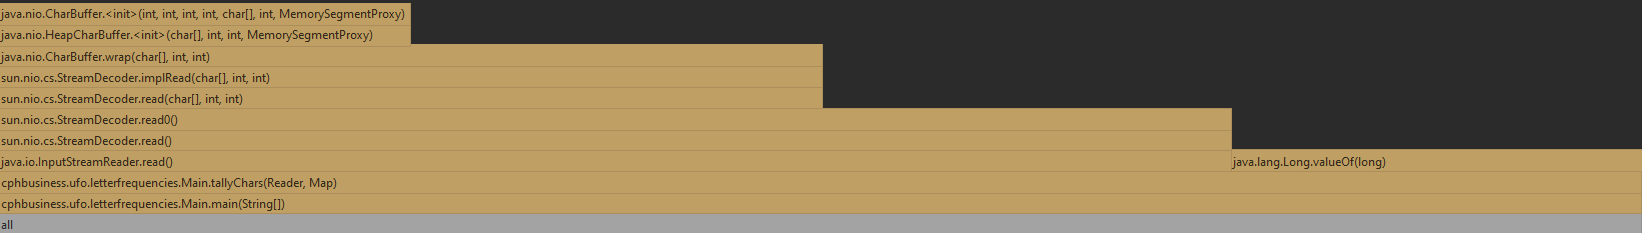
\includegraphics[width=\linewidth]{figures/java_profiler_unchanged_1.png}
    \label{fig:flame-chart-unchanged}
\end{figure}

\begin{figure}[h]
    \caption{Profiler Call Tree}
    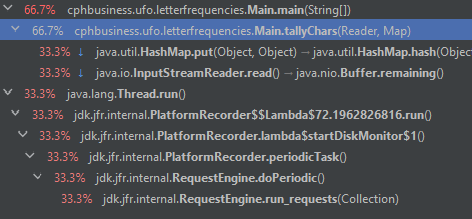
\includegraphics[width=\linewidth]{figures/java_profiler_unchanged_2.png}
    \label{fig:call-tree-unchanged}
\end{figure}

Looking at the charts, we clearly see that the "tallyChars" method  is the most costly function.\\\\
We ran the timer on the method 10 times and got an average of around 4.5ms, which is fairly high compared to other methods, therefor we decided to look further into it.

\newpage

\subsection{Hyphotesis - why is tallyChart so expensive}
The method is using a "Reader" to read data from a text file, which in our experience can be a costly method to run.
After an hour of extensively searching the internet, we came across a reputable source which explained that:

\begin{displayquote}
The new JDK 1.1 improves I/O performance with the addition of a collection of Reader and Writer classes. The readLine method in BufferedReader is at least 10 to 20 times faster than the one in DataInputStream when a large file is encountered. \parencite{how-to-improve-javas-io-performance}
\end{displayquote}

We replaced the old "Reader" with the new "BufferedReader" and gave it a max resource of 10.000 to satisfy it.  
\begin{figure}[h]
    \caption{Main.java with changed Reader type}
    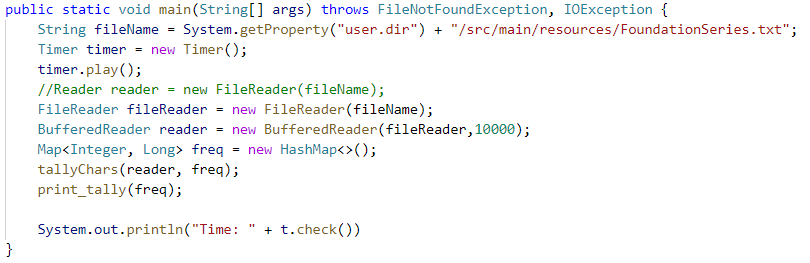
\includegraphics[width=\linewidth]{figures/Figure-3.png}
    \label{fig:flame-chart-unchanged}
\end{figure}

\begin{figure}[h]
    \caption{Main.java with updated tallyChars arguments}
    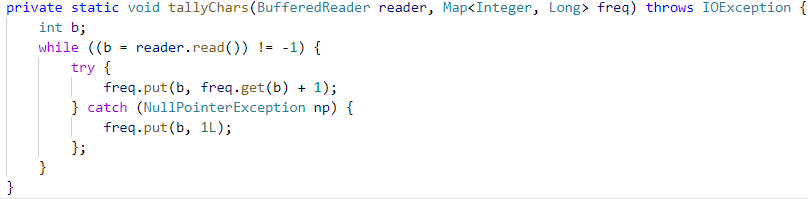
\includegraphics[width=\linewidth]{figures/Figure-4.png}
    \label{fig:flame-chart-unchanged}
\end{figure}

We performed the same test again with a marginal increase in performance.
\begin{lstlisting}[]
Run 1:  82.226 ms
Run 2:  34.3938 ms
Run 3:  58.0026 ms
Run 4:  40.7641 ms
Run 5:  30.4765 ms
Run 6:  39.6008 ms
Run 7:  41.5937 ms
Run 8:  42.4653 ms
Run 9:  52.4299 ms
Run 10: 39.8449 ms    
    \end{lstlisting}